
\documentclass[12pt,twoside]{article}
\usepackage{amsmath}
\usepackage{amssymb}
\usepackage{listings}
\usepackage{color}
\usepackage{graphicx}
\usepackage{parskip}
\usepackage{hyperref}
\usepackage{csvsimple}
\usepackage{siunitx,array,booktabs}


\pagestyle{myheadings}
\textwidth 160mm
\textheight 220mm
\oddsidemargin -.2cm
\evensidemargin -.2cm
\markboth{{\rm G.Drummond, R.Cox}}{{\rm {COSC364 Assignment 1}}}


\begin{document}
\title{COSC364 Assignment 2}
\author{George Drummond(53243258), \\Ryan Cox(64656394)}
\maketitle
\thispagestyle{empty}

\begin{abstract}
The following pertains to COSC364-17S1  Assignment 2.
This was a joint work by George Drummond and Ryan Cox in accordance with the course requirements of COSC364-17S1 and is a result of \bf{equal} contribution ($50\% / 50\%$).
\end{abstract}

\tableofcontents

\newpage
\section{Problem formulation}
We wish to formulate an optimization problem for generic values of X, Y and Z (with $ Y> 3$) such that the load on all transit nodes is balanced. Here we outline the governing mathematical expressions concerning the objective function, the decision variables and all other constraints. The constraints generated by equations \ref{first} through to \ref{last} suffice to fully describe our optimisation problem.

\emph{Notation}: $[X] = \{1,2,3,....,X\}$.

\subsection{Decision and auxiliary variables}
Let $u_{ik}$ be the total amount of flow on the link between a given source node $S_i$ and transit node $T_k$.
Likewise let $v_{kj}$ be the total amount of flow on the link between a given transit node $T_k$ and destination node $D_j$.

Therefore, letting $x_{ikj}$ be the part of the demand volume between source node $S_i$ and destination node $D_j$ that is routed through transit node $T_k$, we achieve 
\begin{align}\label{first}
	u_{ik} &= \sum_{j=1}^{Z}x_{ikj}\\
	v_{kj} &= \sum_{i=1}^{X}x_{ikj}
\end{align}
$\forall i \in [X], k \in [Y], j \in [Z]$.

Also, the total traffic flow into a transit node is equal to the total traffic flow out of the node, achieving the following balance.
\begin{equation}
	\sum_{i=1}^{X}u_{ik} = \sum_{j=1}^{Z}v_{kj}
\end{equation}
$\forall k \in [Y]$.



\subsection{Objective function}\label{Sec: objf}
The goal of this linear program is to balance the load (total \emph{incoming} traffic) across the transit nodes $T_1,T_2,...,T_Y$. As the load on a given transit node $l_k$ is simply the sum of the flows from all source nodes to $T_k$, we achieve
\begin{align*}
	l_k  = \sum_{i=1}^{X}u_{ik},   \quad  \forall k \in [Y]
\end{align*}
As demonstrated in the small example of figure \ref{131}.
\clearpage
\begin{figure}[htb]
	\centering
	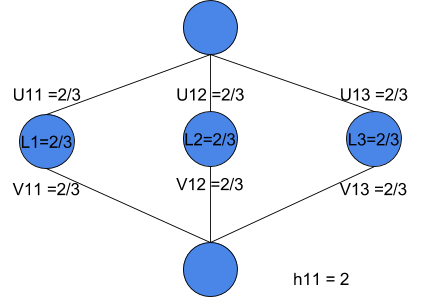
\includegraphics[width=0.5\textwidth]{131.png}
	\caption{X=1,Y=4,Z=1}
	\label{131}
\end{figure}%

At this stage, it may be tempting to define the objective function $l$ as \emph{equal} to all $l_k, \ k \in [Y]$ in order to achieve a common minimum load. This however, would actually lead to an infeasible problem for many cases such as shown in figure\ref{141} below in which all $l_k$ cannot be equal.
%\clearpage
\begin{figure}[htb]
	\centering
	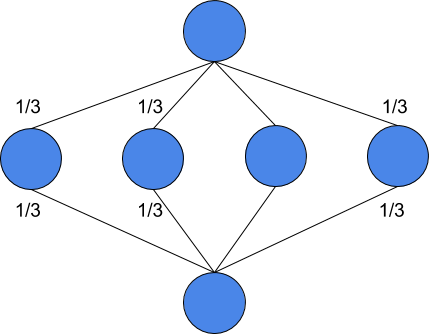
\includegraphics[width=0.5\textwidth]{141.png}
	\caption{X=1,Y=4,Z=1}
	\label{141}
\end{figure}%
%\clearpage

To \emph{balance} this load across the transit nodes, we define our objective function $l$ by
\begin{equation*}
 l = \max{l_k} = \max{\sum_{i=1}^{X}u_{ik}},   \quad  \forall k \in [Y]
\end{equation*}
Proceeding in this fashion acts to minimise the greatest load on a transit node. The piecewise linear interpretation of this is as follows.

\begin{equation}
	l \geq \sum_{i=1}^{X}u_{ik},   \quad  \forall k \in [Y]
\end{equation}



\subsection{Demand constraints}
We now turn our attention to demand constraints and the global requirement that each demand volume $h_{ij}$ between nodes $S_i$ and $D_j$ shall be split over exactly three different paths, such that each path gets an equal
share of the demand volume.

\begin{figure}[htb]
	\centering
	\includegraphics[width=0.5\textwidth]{splitting.png}
	\caption{Splitting requirement}
	\label{splitting}
\end{figure}%

let $w_{ikj}$ be the indicator variable for the path between source node $S_i$ and destination node $D_j$ through transit node $T_k$, taking the value $1$ if path $S_i->T_k->Z_j$ carries data and $0$ otherwise. With our 3 path restriction, we achieve
\begin{equation}
	\sum_{k=1}^{Y}w_{ikj} = 3,   \quad  \forall i \in [X],j \in [Z]
\end{equation}


Now to consider the demand volume between source node $S_i$ and destination node $D_j$. Firstly, we have that this demand volume is simply the sum of the parts of the demand volume through each transit router $T_k,\quad k \in [Y]$.
\begin{equation*}
	\sum_{k=1}^{Y}x_{ikj} = h_{ij}=i+j
\end{equation*}
However, we also have that $x_{ikj}$ will be non-zero if and only if there is flow on path $S_i->T_k->Z_j$ ($w_{ikj} = 1$). As this occurs for precisely 3 $x_{ikj}$ (say $x_{ik_1j}, x_{ik_2j}, x_{ik_3j}$) and the demand $h_{ij}$ is shared \emph{equally} across the paths that do possess flows, we achieve the following.
\[
x_{ikj}  = \left\{\begin{array}{lr}
\frac{(i + j)}{3}, & \text{if } w_{ikj} = 1\\
0, & \text{if } w_{ikj} = 0
\end{array}\right\}
\]
Or explicitly.
\begin{equation}
	x_{ikj} = w_{ikj} \frac{h_{ij}}{3} = \frac{(i + j)}{3}w_{ikj},\quad  \forall i \in [X],k \in [Y],j \in [Z]
\end{equation}



\subsection{Additional constraints}\label{Sec: Const} 
\b{Capacity}:\\
$\forall i \in [X], k \in [Y], j \in [Z]$, we have,
\begin{align}
	u_{ik} &\leq c_{ik} \\
	v_{kj} &\leq d_{kj}  
\end{align}


Non-negativity:\\
$\forall i \in [X], k \in [Y], j \in [Z]$, we have,
\begin{align}
	x_{ikj} &\geq 0\\
	u_{ik} &\geq 0\\
	v_{kj} &\geq 0\\
	l &\geq 0 \label{last}
\end{align}

\section{Results}
The following are the results for fixing X=7, Z = 7 and varying $Y \in {\{3,4,5,6,7\}}$.\\
\begin{center}
	\csvautobooktabular{record.csv}
\end{center}

\section{Discussion}
We can see that as we add more transit nodes between the source and destination nodes that generally the time taken to solve the LP file increases. Also, adding more transit nodes rightly reduces the maximum load. The highest capacity link seems to stay the same as we are only changing the amount of transit nodes the link capacity stays the same and only when we add more nodes does the capacity decrease 










\definecolor{codegreen}{rgb}{0,0.6,0}
\definecolor{codegray}{rgb}{0.5,0.5,0.5}
\definecolor{codepurple}{rgb}{0.58,0,0.82}
\definecolor{backcolour}{rgb}{0.95,0.95,0.92}

\lstdefinestyle{mystyle}{
	backgroundcolor=\color{backcolour},   
	commentstyle=\color{codegreen},
	keywordstyle=\color{magenta},
	numberstyle=\tiny\color{codegray},
	stringstyle=\color{codepurple},
	basicstyle=\footnotesize,
	breakatwhitespace=false,         
	breaklines=true,                 
	captionpos=b,                    
	keepspaces=true,                 
	numbers=left,                    
	numbersep=5pt,                  
	showspaces=false,                
	showstringspaces=false,
	showtabs=false,                  
	%tabsize=2
}

\lstset{style=mystyle}

\newpage

\section{Appendix}
\subsection{LP generation source file}
\lstinputlisting[language=python]{genLP.py}
\newpage
\subsection{LP File for X = 3, Y = 2 and Z = 4}
\lstinputlisting{324.lp}



\end{document}



%%%%%%%%%%%%%%%%%%%%%%%%%%%%%%%%%%%%%%%%%% Non-relevent stuff below this line %%%%%%%%%%%%%%%%%%%%%%%%%%%%%%%%%%%%%